\section{Tangents and Normals}

\subsection{Tangent Lines to Level Curves}

If $\vec{r} = g(t)\hat{i} + h(t)\hat{j}$ is a smooth curve on the level curve $f(x, y) = c$ of a differentiable function $f$, then
\begin{align*}
    f(g(t), h(t)) &= c \\
    \frac{d}{dt} f(g(t), h(t)) &= \frac{d}{dt}(c) \\
    \frac{\del f}{\del x} \frac{dg}{dt} + \frac{\del f}{\del y} \frac{dh}{dt} &= 0 \\
    \llangle \frac{\del f}{\del x}, \frac{\del f}{\del y} \rrangle \cdot \llangle \frac{dg}{dt}, \frac{dh}{dt} \rrangle &= 0 \\
    \grad f \cdot \frac{d\vec{r}}{dt} &= 0
\end{align*}

This essentially means that the gradient of $f$ is always normal to the tangent at a level curve, which makes sense as
gradient describes the change, whereas the level curve describes the \textit{constant-ness}.

The line through a point $P_0 = \point$ normal to a vector $\vec{n} = A\hat{i} + B\hat{j}$ has the equation
\begin{equation}
    A(x - x_0) + B(y - y_0) = 0
\end{equation}

And if $\vec{n}$ is the gradient $(\grad f)_{\point} = f_x\point\hat{i} + f_y\point\hat{j}$,
the equation of the tangent line is given by
\begin{equation}
    f_x\point (x - x_0) + f_y \point (y - y_0) = 0
\end{equation}

\begin{example}
    \normalfont Find the equation of the tangent to the given ellipse at $(-2, 1)$.
    $$\frac{x^2}{4} + y^2 = 2$$

    Note that the given ellipse is a level curve of $f(x, y) = \frac{x^2}{4} + y^2$. Then, at $(-2, 1)$,
    $$ (\grad f)_{(2, -1)} = \llangle \frac{x}{2}, 2y \rrangle_{(-2, 1)} = \langle -1, 2 \rangle $$

    Hence, the tangent to the ellipse at $(-2, 1)$ is given by
    \begin{align*}
        -1 (x - (-2)) + 2 (y - 1) &= 0 \\
        x - 2y &= -4
    \end{align*}
\end{example}


\subsection{Tangent Planes to Level Surfaces}
If $\vec{r} = g(t)\hat{i} + h(t)\hat{j} + k(t)\hat{k}$ is a smooth curve on the level urface $f(x, y, z) = c$ of a differentiable
function $f$, then
\begin{align*}
    f(g(t), h(t), k(t)) &= c \\
    \frac{d}{dt} f(g(t), h(t), k(t)) &= \frac{d}{dt}(c) \\
    \frac{\del f}{\del x} \frac{dg}{dt} + \frac{\del f}{\del y} \frac{dh}{dt} + \frac{\del f}{\del z} \frac{dk}{dt} &= 0 \\
    \llangle \frac{\del f}{\del x}, \frac{\del f}{\del y}, \frac{\del f}{\del z} \rrangle \cdot
    \llangle \frac{dg}{dt}, \frac{dh}{dt}, \frac{dk}{dt} \rrangle &= 0 \\
    \grad f \cdot \frac{d\vec{r}}{dt} &= 0
\end{align*}

Analagous to \textit{tangent lines to level curves}, this means that the tangent at a level curve is always normal to the
gradient at any point. So, if $\vec{n}$ is the gradient $(\grad f)_{P_0} = f_x(P_0)\hat{i} + f_y(P_0)\hat{j} + f_z(P_0)\hat{k}$
for some $P_0 = (x_0, y_0, z_0) \in \R^3$, then the equation of the tangent plane is given by

\begin{equation}
    f_x(P_0)(x - x_0) + f_y(P_0)(y - y_0) + f_z(P_0)(z - z_0) = 0
\end{equation}

Thus, the tangent plane at a point $P_0$ on the level surface $f(x, y, z) = c$ is a plane normal to $(\grad f)_{P_0}$.


\subsection{Normal Line to Level Curves and Surfaces}
The normal line to a level curve $f(x, y) = c$ at a point $P_0 = \point \in \R^2$, or to a level surface $f(x, y, z) = c$ at a point
$P_0 = (x_0, y_0, z_0) \in \R^3$, is a line through $P_0$ parallel to $(\grad f)_{P_0}$. In three dimensions, the equation
of the normal is given by

$$x = x_0 + f_x(P_0) t, \ \ \ y = y_0 + f_y(P_0) t, \ \ \ z = z_0 + f_z(P_0) t$$

\begin{figure}[htp]
    \centering
    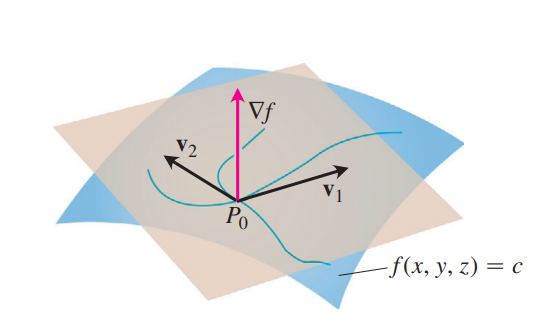
\includegraphics[scale=0.45]{tangent-normal.png}
    \caption{The gradient $\grad f$ is orthogonal to the tangent plane of a level surface}
\end{figure}

\begin{example}
    \normalfont Find the tangent plane and normal line of the surface $f(x, y, z) = x^2 + y^2 + z - 9 = 0$ at the point
    $P_0 = (1, 2, 4)$.

    We first find the gradient of $f$:
    $$(\grad f)_{P_0} = \langle 2x, 2y, 1 \rangle_{P_0} = \langle 2, 4, 1\rangle$$

    Hence, the equation of the tangent plane is
    \begin{align*}
        2 (x - 1) + 4 (y - 2) + 1 (z - 4) &= 0 \\
        2x + 4y + z &= 14
    \end{align*}

    For the equation of the normal line at $P_0$, we have
    $$\frac{x - 1}{2} = \frac{y - 2}{4} = z - 4$$
\end{example}

\begin{example}
    \normalfont The surfaces $f(x, y, z) = x^2 + y^2 - 2 = 0$ (a cylinder) and $f(x, y, z) = x + z - 4 = 0$ (a plane)
    meet in an ellipse $E$. Find the parametric equations for the line tangent to $E$ at $P_0 = (1, 1, 3)$.

    \begin{figure}[htp]
        \centering
        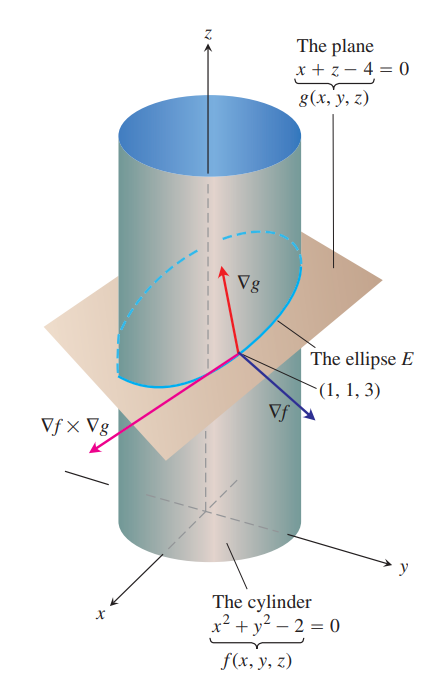
\includegraphics[scale=0.5]{example-8.3.2.png}
        \caption{Intersection of Cylinder $f(x, y, z) = 0$ and Plane $g(x, y, z) = 0$}
    \end{figure}

    Note that the tangent to $E$ is orthogonal both to the gradient of the cylinder, $\grad f$, and the gradient
    of the plane, $\grad g$. Hence, the tangent is parallel to $\vec{v} = \grad f \times \grad g$.

    \begin{align*}
        (\grad f)_{P_0} &= \langle 2x, 2y, 0 \rangle_{P_0} = \langle 2, 2, 0 \rangle \\
        (\grad g)_{P_0} &= \langle 1, 0, 1 \rangle_{P_0} = \langle 1, 0, 1\rangle \\
        \vec{v} &= \langle 2, 2, 0 \rangle \times \langle 1, 0, 1 \rangle =
        \begin{vmatrix}
            \hat{i} & \hat{j} & \hat{k} \\
            2 & 2 & 0 \\
            1 & 0 & 1
        \end{vmatrix} = 2\hat{i} - 2\hat{j} - 2\hat{k}
    \end{align*}

    Hence, the parametric equation of the line is
    $$x = 1 + 2t, \ y = 1 - 2t, \ z = 3 - 2t, \text{  or  } \vec{r} = (\hat{i} + \hat{j} + 3\hat{j}) +
    \lambda (\hat{i} - \hat{j} - \hat{k})$$
\end{example}